\documentclass[11pt]{article}
\usepackage[longtitle]{emergentwisdom-preprint}
\usepackage{amsmath,amssymb}
\usepackage{booktabs}
\usepackage{tabularx}
\usepackage{array}
\usepackage{enumitem}
\usepackage{microtype}
\usepackage{xcolor}
\usepackage{tikz}
\usetikzlibrary{arrows.meta,positioning,fit,calc}
\usepackage{float}
\usepackage{cite}
\usepackage{hyperref}

\definecolor{ewblue}{HTML}{24527A}
\definecolor{ewteal}{HTML}{2D7C78}
\definecolor{ewgold}{HTML}{A76F16}
\definecolor{ewgray}{HTML}{F2F4F6}

\hypersetup{
  hidelinks,
  pdftitle={Imagining the Corpus: Turning Text into Video for Language Model Training},
  pdfauthor={Henrik Westerberg},
  pdfsubject={A proposal to turn the text corpus into synchronized explanatory video and train language models to predict text and video together},
  pdfkeywords={imagining the corpus, corpus-to-video compilation, document-to-world compilation, synthetic training data, video-language modeling, persistent world modeling, joint prediction, mental imagery, representation learning, teacher-augmented distillation}
}

\makeatletter
\renewcommand{\@openbib@code}{\setlength{\itemsep}{0pt}\setlength{\parsep}{0pt}}
\makeatother

\title{Imagining the Corpus:\\Turning Text into Video for Language Model Training}
\renewcommand{\shorttitle}{Imagining the Corpus}
\author{Henrik Westerberg\\Emergent Wisdom\\
  \texttt{henrik.westerberg@emergentwisdom.org}}
\ewreviseddates{August 26, 2026}{November 8, 2026}

\newcommand{\record}{\mathcal{Q}}
\newcommand{\compiler}{\mathcal{C}}
\newcommand{\loss}{\mathcal{L}}

\raggedbottom
\begin{document}
\maketitle

\begin{abstract}
Language models learn from text, but text omits much of the spatial, physical, causal, and conceptual structure that readers reconstruct. This paper proposes a new pretraining paradigm: turn the text corpus into synchronized video, then train a language model to predict both the exact native text and its evolving visual world. A prefix-causal compiler preserves every source span while creating persistent trajectories across whole documents. Fiction can become continuous scenes; mathematics, code, protocols, and scientific mechanisms can become animated notation, proof, execution, or schematic processes. The distinctive target is the \emph{unvisualized abstract corpus}: synthetic, temporally evolving representations of knowledge for which no adequate video exists, optimized for learner utility rather than cinematic realism. The highest ambition is corpus-wide video, with every part of the training text paired with a temporally evolving explanatory world. Keyframes, sparse animation, diagrams, and visual latents form cheaper visual rungs that may already yield gains and reveal what full video must preserve; registries and controlled descriptions provide structured scaffolds and matched baselines. One shared block-causal language model predicts the next text span, visual interval, and registry update from their completed histories. Source-only compilation reorganizes relations supported by the text. Teacher-augmented compilation can also transfer perceptual and physical regularities from renderers trained on real images or video, external evidence from retrieval, and checked structure from simulators or formal tools. The central hypothesis is that learning to continue language and explanatory video together can make constraints, consequences, and reusable transformations more accessible to a finite learner. Matched controls and directed interventions test whether the added track is causally used. Corpus-wide video would be enormously expensive today, but declining costs could justify it if smaller experiments show a capability that cheaper text-only training cannot provide. This paper defines the pipeline and its tests; it reports no such evidence.
\end{abstract}

\keywords{Imagining the Corpus, Corpus-to-Video Compilation, Document-to-World Compilation, Synthetic Training Data, Video-Language Modeling, Persistent World Modeling, Joint Prediction, Mental Imagery, Representation Learning, Teacher-Augmented Distillation}

\section{Introduction}

The central proposal is to turn the text corpus into synchronized video and train a language model to continue both. A compiler works through fiction, nonfiction, mathematics, code, and other documents in order, preserves every native text span, and constructs an evolving visual counterpart that accompanies it: a world, mechanism, proof, execution, or conceptual process. One shared predictive model then learns the next exact text and the next video interval together. In its shortest form, the proposal is: \emph{turn all text into video, then make prediction of that video part of learning the text}. This is not a separate film archive placed beside a language model. It is a pipeline for creating a new training target and a new kind of language model while retaining the predictive training path that already works at scale.

Here \emph{mental imagery} is a functional analogy, not a claim about consciousness or a reconstruction of private human experience. It means an externalized visual, spatial, temporal, diagrammatic, or simulated representation that could support understanding. The useful representation need not be the one a person finds most intuitive. Its value is determined by whether its intended structure causally improves prediction, consistency, transfer, or problem solving for the learner.

Human cognition and practice supply a motivating precedent for this organizational hypothesis. During conceptual problem solving, some people construct and manipulate schematic spatial images, while others rely on pictorial imagery or show no consistent preference for imagery~\cite{kozhevnikov2002visualizer}; this is a documented strategy, not a universal model of thought. Informationally equivalent diagrams can reduce search and make relations explicit that remain costly to recover from prose, while actions in an external environment can simplify problems that are harder to solve mentally~\cite{larkin1987diagram,kirsh1994epistemic}. Analogy and metaphor can likewise map relational structure from a familiar domain into an unfamiliar one without being literally visual~\cite{gentner1983structure}. People create such aids selectively and intermittently; the proposed compiler asks whether a learner can instead maintain and predict source-grounded literal or schematic states, together with separately typed constructed analogies, throughout a document. Emitting these representations is not itself evidence of reasoning: the causal tests below must show that their structure changes later prediction or manipulation in the expected direction.

This remains a language model in the ordinary predictive sense. It uses the same native text as a next-token model, preserves its order and wording, and keeps future language as an output. Compilation adds a synchronized visual continuation target rather than replacing the book. For a story, video may show a changing physical scene; for mathematics, animated notation, geometry, dependencies, or proof state; for software, changing code, memory, data flow, terminal output, or interface state. Here \emph{video} means an evolving visual representation, not only photorealistic cinema. Its content can optimize for persistence, constraint exposure, and useful structure rather than literal recognizability alone.

The proposal therefore extends beyond filming what could already be seen. It asks what it would mean to watch a proof about topological invariants, a distributed-systems protocol, or a neuroscience synthesis unfold while it is read. Such trajectories might show objects transforming while invariants persist; messages, failures, and local states evolving through a protocol; or causal processes crossing molecular, cellular, circuit, and behavioral scales. Few such records exist, and people could not feasibly author them across the corpus. A sufficiently capable compiler could propose and compare literal, schematic, metaphorical, and machine-native trajectories, creating synthetic training data whose representational relationships have never been externalized at corpus scale. The criterion is not whether a person would have made or immediately recognized the video, but whether its declared structure is auditable and makes relevant constraints or transformations causally more useful to the learner.

Compilation can change training in two ways. Source-only records reorganize relations already supported by the completed text. Teacher-augmented records can also transfer knowledge acquired outside the text. A renderer trained on real images or video can carry perceptual and physical regularities into the synthesized trajectory. Retrieval can supply external evidence, while simulators, theorem provers, and execution tools can contribute mechanically checked structure. Formal tools can remain source-only when they only apply a preregistered transformation entailed by the prefix. In schematic form, sensory or formal experience enters a teacher, the teacher constructs synchronized explanatory targets, and those targets become part of language-model training. This is a cross-modal and formal distillation route, although the same route can also transmit errors and artifacts.

Corpus-wide video is the most expansive visual version of the proposal because a temporally resolved world can carry identity, geometry, motion, mechanism, intermediate state, invariant, and consequence together. Lower-cost visual targets remain scientifically important. Keyframes, sparse animation, animated diagrams, proof or execution visualizations, and visual latents may already improve learning, reveal which relations matter, and make an early experiment feasible. Registries and persistent descriptions provide structured scaffolds and matched baselines. These alternatives form an empirical route toward the full ambition rather than competing definitions of the paper. The testable claim is narrower than the vision: under matched controls, the added track should improve state tracking, consistency, transfer, composition, or problem solving, and controlled edits should change later predictions in the direction their content implies.

The proposal continues the research program of the Substrate-Translated Language Model (STLM)~\cite{westerberg2026stlm}. STLM asks whether every lexical decision can be made to pass through an externally structured substrate. Its continuous Stage~5 retains two serial networks: a substrate predictor updates a continuous scene, and a token readout receives only that predicted state. This paper uses a different routing design. One shared block-causal model receives completed text, scene, and registry history and predicts the next text span, scene interval, and registry update in parallel. The scene is not a compulsory bottleneck, so the design preserves a direct language-history route and parallel supervision but gives up STLM's architectural guarantee. It is not necessarily easier or cheaper to implement or train.

The relation to Entangled Alignment is a relation between two analytically separable but potentially overlapping omissions in the training record. The Missing Reader is the absent continuous reader position and under-recorded update policy through which noticing, questioning, evaluating, and revising unfold~\cite{westerberg2026entangled}. The missing imagery is the absent visual or schematic state through which a situation, mechanism, proof, or program could be represented. Both can be generated synthetically, but neither is claimed to recover an original person's hidden cognition. A source-supported depiction belongs to the world track; an imagined alternative or reader-constructed transformation belongs to the optional reader track. Section~\ref{sec:reader-track} keeps these roles separate.

Some suitable training records already exist. Films combine persistent events with dialogue; documentaries and demonstrations combine narration with visible processes; technical animations combine explanations with moving diagrams. Unified multimodal models already predict text and visual elements in shared sequences or objectives~\cite{videobert,emu,emu35,tv2tv}. But temporal co-occurrence is not the same as depicting what language means. A talking-head video may reveal identity, expression, and turn-taking while showing almost nothing about the mechanism or abstract idea under discussion. Much of the knowledge in books, mathematics, and code has no suitable video at all.

Corpus-to-video compilation fills that gap. A compiler preserves every exact source span, maintains recurring entities and state, creates a persistent visual trajectory, and records how source events correspond to its intervals. The resulting video is training data: its purpose is to become a co-evolving prediction target for the language model, not only a human-viewable adaptation.

The core contribution is the combination of four elements:

\begin{enumerate}[leftmargin=1.6em,itemsep=2pt,topsep=3pt]
  \item a new corpus-level synthetic-data target: persistent explanatory video synchronized with the complete sequence of exact native source spans, including machine-optimized visualizations of abstract concepts and mechanisms for which no adequate video counterpart exists;
  \item an exact-source-preserving, prefix-causal compiler and a visual representation ladder from keyframes, sparse animation, diagrams, and visual latents to continuous corpus-wide video, with a relation-first policy for deciding what each visual trajectory must preserve and registry and description scaffolds for attribution;
  \item one shared block-causal language model that predicts native text, the selected visual or schematic target, and registry updates together, allowing constraints learned in either form to influence the common predictive state; and
  \item an explicit separation between source-only reorganization and teacher-augmented knowledge transfer, together with matched controls that test whether persistent explanatory history is causally used rather than merely predicted.
\end{enumerate}

Scene-consistency checking, reliance training, routing, and reader-side imagery are optional realization and evaluation ideas. They are not required to define the corpus-to-video pipeline.

The paper specifies a research program rather than a completed model or corpus. Its scene-history claim succeeds only if scene history has a content-specific effect beyond matched scene-target supervision and persistent descriptions, and directional tests show that text and scene constrain one another. Registry-only gains remain complete-pipeline effects unless an analogous registry-target control is added.

\section{Existing Training Data and the Missing Coverage}
\label{sec:natural}

Language is an incomplete sensory record. A sentence such as ``the cup fell'' specifies an event but normally leaves trajectory, orientation, collision geometry, and many consequences unstated because readers are expected to bring learned perceptual and physical knowledge. Congenital blindness provides an important boundary case. People born blind can acquire fine-grained distinctions among visual and light verbs and broadly typical action-concept structure without first-person vision~\cite{bedny2012action,bedny2019sparkle}. Yet visual experience can still affect how a visually diagnostic relation---for example, color similarity among fruits and vegetables---organizes implicit conceptual similarity~\cite{connolly2007blindness}. This does not imply that vision is necessary for language or intelligence. It motivates the narrower question here: can a compiled explanatory track make some structure that prose leaves implicit easier for a finite learner to recover and use?

Natural video-language records provide the cheapest first test because they avoid errors from synthetic rendering. Their usefulness depends on whether visible change bears on the accompanying language.

\begin{center}
\begin{tabularx}{0.97\linewidth}{@{}>{\bfseries}p{0.23\linewidth}p{0.36\linewidth}X@{}}
\toprule
Source & Useful signal & Main limitation \\
\midrule
Film or enacted narrative & Persistent people, places, objects, actions, and consequences & Dialogue and subtitles do not describe everything visible; adaptations omit and rearrange source material \\
Documentary or narrated demonstration & Language paired with organisms, environments, tools, actions, and physical processes & Narration can be delayed, incomplete, or concerned with something off-screen \\
Technical animation or diagram-led lecture & Equations, diagrams, mechanisms, procedures, and changing formal state & Visuals can be static, decorative, or only loosely synchronized with the explanation \\
Talking head or interview & Identity, gesture, affect, gaze, and conversational intent & Usually does not depict the external system or abstract subject under discussion \\
Compiled document & Purpose-built, persistent depiction or schematic state paired with exact source text & The world track is synthetic and inherits compiler and renderer errors \\
\bottomrule
\end{tabularx}
\end{center}

Large narrated-video corpora and structured interleaved datasets establish that useful paired records can be collected at scale~\cite{howto100m,multimodaltextbook,comm}. VideoBERT, Emu, Emu3.5, and TV2TV establish increasingly direct precedents for learning from temporally interleaved text and visual sequences~\cite{videobert,emu,emu35,tv2tv}. These systems motivate a natural-data phase in which one shared model predicts both tracks and researchers shift or remove each history track to measure dependence.

A Stage-0 natural-data experiment should compare aligned records with three matched controls: removed visual history, temporally shifted or cross-record visual history, and a visual-only learner without language history. The same trained capacity and evaluation set should be used to score both next-language and next-scene prediction. This establishes whether the joint objective creates bidirectional predictive dependence before synthetic compilation adds its own errors.

Natural data cannot cover the proposal's intended domain. Explanatory video is sparse relative to text, adaptations do not preserve every sentence, and most abstract knowledge is not recorded as a changing scene. Compilation therefore uses existing explanatory media in two ways: directly as initial training data and indirectly as examples of how language can be converted into useful visual or schematic state. The synthetic track should depict the subject of the text, not merely decorate it.

\section{A Representation Ladder toward Corpus-Wide Video}
\label{sec:representation-selection}

The representation program is hierarchical. Its most expansive visual target is persistent video for the complete corpus: an evolving visual world synchronized with every source event across a document. Full video need not be the first practical experiment, and it is not assumed to win before testing. Keyframes, sparse animation, animated diagrams, symbolic-spatial visualizations, and visual latents provide cheaper visual rungs. Registries and controlled descriptions remain separate structured scaffolds and matched baselines. A positive result on any lower-cost condition is useful in its own right and can identify structure that a later video system should preserve. The ladder orders temporal density, generation cost, and proximity to the corpus-wide video ambition; it does not assume monotonic capability. A diagram, proof state, execution trace, or latent may ultimately outperform dense video for a particular domain.

Even within the video ambition, a passage does not determine one uniquely useful rendering. The same physical event may be represented as cinematic motion, sparse animation, changing keyframes, or an object--relation diagram unfolding over time. A mathematical argument may become animated notation, geometry, a dependency graph, or a proof state; a program may become changing source, data flow, memory, terminal output, or an interface trace. These choices expose different regularities and impose different prediction costs.

Abstract compilation should not be restricted to inherited explainer-video conventions. Candidate trajectories may use unfamiliar spatial mappings, nonphotorealistic motion, constructed metaphors, or learned visual--symbolic dynamics. Machine-native does not mean exempt from evaluation: each condition must preserve preregistered relations, survive matched controls and directional interventions, and improve a declared endpoint. Constructed analogies remain typed as analogies so that a useful metaphor is not mistaken for a source fact.

At corpus scale, consistency becomes another experimental variable. A representation policy can reuse visual primitives for recurring relations across documents, allowing a successful metaphor to become a shared notation rather than a one-off illustration. Compare corpus-consistent motifs with document-local and permuted assignments; only transfer to held-out relations, domains, or compositions credits the shared visual vocabulary.

The search should begin with relations rather than rendering style. Before choosing dense pixels, sparse frames, a diagram, a latent, or a structured nonvisual control, an experiment should specify the most general relations that the source and evaluation require the learner to preserve---for example identity, geometry, causality, invariants, control flow, or epistemic status. These are candidate dimensions, not a fixed ontology. Candidate externalizations should preserve the same declared relations where possible, and every relation present in only one family must be recorded. Otherwise a comparison confounds representational organization with information content.

\begin{samepage}
Consider one exact source event: ``Lea tilted the blue tray, so the brass key resting on it slid onto the floor.'' The compiler can externalize the same event in several forms that can be appended to persistent history:

\begin{center}
\small
\begin{tabularx}{0.97\linewidth}{@{}>{\raggedright\arraybackslash\bfseries}p{0.20\linewidth}p{0.39\linewidth}X@{}}
\toprule
Externalization & Event state & What it exposes \\
\midrule
Registry $R$
& Stable IDs $k$ (brass key) and $t$ (blue tray); $\operatorname{on}(k,t)$ before the event; a causal edge $\operatorname{tilt}(t)\!\rightarrow\!\operatorname{slide}(k)$; and $\operatorname{on}(k,\mathrm{floor})$ afterward
& Explicit, readily queryable identity, causal linkage, and discrete before--after relations, but no continuous geometry. \\
Persistent description $D$
& ``Key $k$ was supported by tray $t$; $t$ rotated to a tilted pose, causing $k$ to move continuously from its prior position until it contacted the floor.''
& The same declared identity, causal order, transition, and motion relations as the scene, in linguistic form. Source-underdetermined details remain marked as inferred. \\
Literal scene $V^{\mathrm{lit}}$
& A short clip or keyframe sequence with stable assets for $k$ and $t$, the changing tray angle, the key's path, and floor contact
& The declared geometry and motion relations, together with nuisance values for viewpoint and rendering that the source does not determine. \\
Causal diagram $V^{\mathrm{causal}}$
& $\operatorname{tilt}(t)\rightarrow\operatorname{slide}(k)\rightarrow\operatorname{on}(k,\mathrm{floor})$
& Causal order and candidate intervention points while discarding surface appearance; counterfactual consequences still require transition semantics. Any unstated mechanism must remain marked as inferred. \\
\bottomrule
\end{tabularx}
\end{center}
\end{samepage}

These are not interchangeable pictures of one complete ground truth. They preserve some common relations while making different structure cheap to recover. The experiment asks which externalization enables a finite learner to predict or manipulate the relevant relation, not which one appears most vivid to a person.

Representation family and rung are therefore experimental variables rather than aesthetic preferences. Candidate literal scenes, explanatory diagrams, animations, symbolic-spatial states, execution traces, latents, and linguistic controls should first be compared on small controlled domains built from the same source content and verified underlying state. Generation and decodability alone do not make a representation useful to a learner. Its intended structure must produce a task-specific causal benefit under matched controls. Human legibility remains useful for auditing and intervention, but human visual appeal is not the optimization target.

Let $V_e^{(r)}$ denote representation family $r$'s rendering of the same source event and verified registry state. Screening estimates utility by task rather than imposing one total ordering; the selected family and policy version are subsequently recorded in $P_e$.

For each representation family, the first screen should compare aligned text--registry--scene training with text plus registry but no scene, a scene-target-only condition without scene history, text plus scene but no model-visible registry, aligned registry with a matched wrong scene, a linguistic description-target control, and a persistent-description-history control encoding the same declared relations. Text-only and scene-only conditions provide additional anchors. Evaluation should include later-language prediction, state prediction, held-out composition, responses to controlled edits, sample efficiency, and generation and training cost. Target bandwidth, backbone capacity, supervision density, and optimization should be matched where possible; otherwise the result must be reported as a comparison between complete pipelines rather than as a pure effect of representation.

The result may be a conditional video policy rather than one rendering style. Spatial layouts may help spatial inference, animated transitions may help mechanisms, equation and proof-state animation may help mathematics, execution traces may help code, and registries may support identity and long-range consistency beneath the visual track. Document-scale generation should follow this screen. The long-term endpoint remains a synchronized evolving visual trajectory, while lower rungs can be retained wherever they are more useful or economical.

\section{Compiling a Whole Document into a World Trajectory}
\label{sec:compiler}

Let a document be a token sequence $X=(x_1,\ldots,x_N)$. The compiler partitions it into meaning-bearing events and returns
\begin{equation}
  \compiler(X)=\{\record_e\}_{e=1}^{E}, \qquad
  \record_e=(T_e,V_e,\Delta R_e,D_e;A_e,U_e,P_e).
  \label{eq:record}
\end{equation}
Here $T_e=x_{a_e:b_e}$ is an exact immutable source span; $V_e$ is a visual or schematic trajectory; and $\Delta R_e$ updates a persistent registry $R_e$ of entities, attributes, relations, locations, beliefs, variables, and unresolved facts. $D_e$ is a stored derived scene description. The core condition withholds it from the model's input, while the description controls below use it as a target or persistent history. The fields after the semicolon are metadata: $A_e$ records synchronization, $U_e$ records uncertainty and alternatives, and $P_e$ records provenance, licenses, generators, prompts or programs, revisions, and hashes. These metadata are retained for construction and evaluation but are not model inputs or prediction targets in the core condition.

Every record is labeled \emph{source-only} or \emph{teacher-augmented}. In the source-only regime, each task-relevant relation visible in $R_e$, $D_e$, or $V_e$ must be explicit in or entailed by $T_{\le e}$ under a frozen auditable rule set or simulator. This regime tests whether reorganization makes existing source information more usable. Teacher-augmented compilation is a deliberate transfer route, not merely a contaminated source-only record. A renderer trained on real images or video can distill perceptual and physical regularities into the explanatory target. Retrieval can supply external evidence, while simulators, theorem provers, and program execution can contribute mechanically checked structure. A formal tool can remain source-only when it only applies a preregistered transformation entailed by the prefix. Otherwise, unsupported task-relevant additions make the affected fields teacher-augmented and retain field-level provenance. This second regime tests whether sensory or formal knowledge can enter language-model training through synchronized synthetic records. It must be reported separately because the same channel can transmit stereotypes, physical errors, unsupported interpretations, or generator artifacts.

Keeping $U_e$ hidden is an attribution baseline, not the intended mature treatment of ambiguity. An uncertainty-visible extension may expose only a prefix-causal projection $U_e^{\mathrm{pre}}$: unknown or ambiguous status, compiler confidence, and weighted valid alternatives available from $T_{\le e}$. Any label obtained by consulting later source text remains audit metadata and must never enter predictive history.

A stronger ambiguity-aware variant can maintain $B$ weighted, prefix-causal world hypotheses rather than force one interpretation into the record. Each hypothesis must remain coherent across an event, and a generated text--scene--registry bundle must use one branch rather than switch branches between tokens or heads. This is an optional ambiguity-management mechanism. Its cost, branch collapse, and any scene-specific effect beyond matched registry and non-scene fields must be evaluated separately.

For attribution, $R_e$ and $V_e$ are separate channels, and only an incremental or directional effect of $V_e$ beyond matched registry and persistent-description conditions counts as evidence for scene utility. Before training, each experiment must preregister and freeze the registry schema, the fields intentionally excluded from it, and the relations assigned only to the scene. This prevents the boundary between registry and scene from moving after the results are known. Freezing is an attribution rule within an experiment, not a claim that the schema is final. Between experiments, recurring failures may reveal an omitted or badly carved relation. A revised schema must receive a new version, be declared before the next comparison, and be applied to every affected condition; earlier results retain the scope of the schema under which they were obtained.

\begin{figure}[H]
\centering
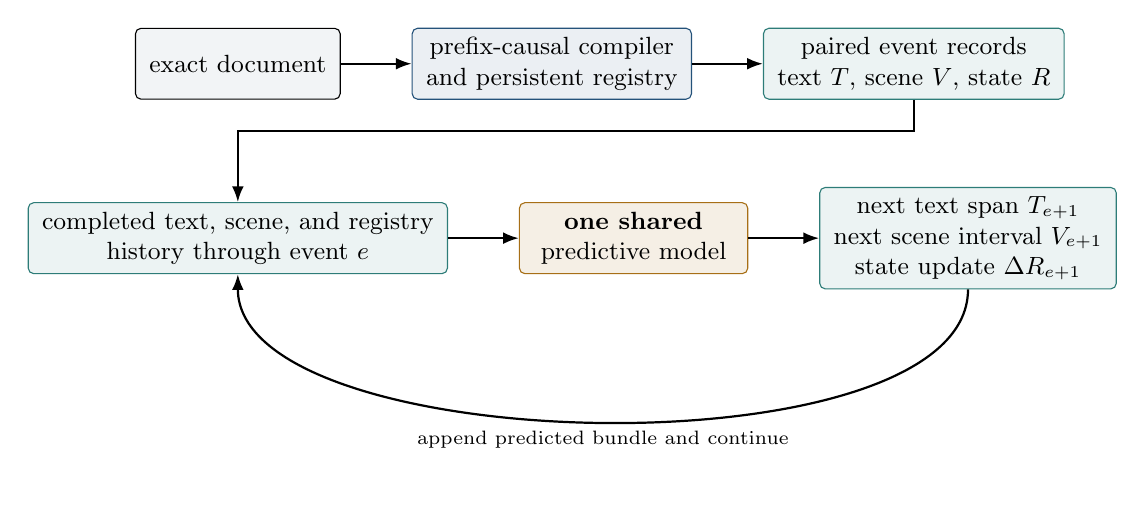
\begin{tikzpicture}[
  node distance=8mm and 9mm,
  box/.style={draw,rounded corners=2pt,align=center,minimum height=9mm,inner xsep=5pt,font=\small},
  source/.style={box,fill=ewgray},
  process/.style={box,fill=ewblue!9,draw=ewblue},
  record/.style={box,fill=ewteal!9,draw=ewteal},
  model/.style={box,fill=ewgold!11,draw=ewgold},
  arrow/.style={-{Latex[length=2mm]},thick}
]
  \node[source] (book) {exact document};
  \node[process,right=of book] (compile) {prefix-causal compiler\\and persistent registry};
  \node[record,right=of compile] (records) {paired event records\\text $T$, scene $V$, state $R$};
  \draw[arrow] (book) -- (compile);
  \draw[arrow] (compile) -- (records);

  \node[record,below=13mm of book] (history) {completed text, scene, and registry\\history through event $e$};
  \node[model,right=of history,minimum width=29mm] (shared) {\textbf{one shared}\\predictive model};
  \node[record,right=of shared] (future) {next text span $T_{e+1}$\\next scene interval $V_{e+1}$\\state update $\Delta R_{e+1}$};
  \coordinate (feed) at ($(records.south)+(0,-4mm)$);
  \draw[arrow] (records.south) -- (feed) -| (history.north);
  \draw[arrow] (history) -- (shared);
  \draw[arrow] (shared) -- (future);
  \draw[arrow] (future) to[out=-90,in=-90,looseness=0.65]
    node[below,font=\scriptsize] {append predicted bundle and continue} (history);
\end{tikzpicture}
\caption{Corpus-to-video compilation and joint continuation. The compiler preserves exact text while constructing persistent explanatory video or a lower-rung trajectory. One shared block-causal model predicts the next native text, visual interval, and registry update from completed paired history.}
\label{fig:pipeline}
\end{figure}

\subsection{One document, several clocks}

A book advances in tokens, meanings, and depicted time rather than at one frame rate. Each event therefore connects a source span to a trajectory interval:
\begin{equation}
  e \longleftrightarrow [a_e,b_e) \longleftrightarrow [\tau_e^0,\tau_e^1).
  \label{eq:synchronization}
\end{equation}
A phrase can govern a long physical transition; a page of exposition can correspond to one slowly changing diagram. The compiler does not need one image per word. It needs explicit event boundaries and persistent identifiers so that later appearances of a person, object, variable, or location refer to the same evolving state.

For causal prediction experiments, earlier records must not contain later revelations:
\begin{equation}
  \record_e=\compiler_e(T_{\le e}), \qquad
  \record_e\not\leftarrow T_{>e}.
  \label{eq:prefixcausal}
\end{equation}
Equation~\ref{eq:prefixcausal} constrains more than the visible prompt. A pretrained compiler or learner may already contain later passages of a familiar book in its weights. Primary causal evaluation should therefore use an auditable compiler and sources known to have been unavailable to every pretrained compiler and learner component, or train those components from documented data. Suitable sources include material created prospectively after checkpoints are frozen and access-controlled private or unpublished material. A full-book renderer may use future text to produce a polished adaptation, but that version cannot test next-event prediction because an earlier frame can encode a later revelation. Teacher-augmented compilation may use licensed external knowledge with field-level provenance, but both regimes must remain blind to $T_{>e}$. Exact-source preservation alone does not make a record source-only.

\subsection{A practical whole-book compiler}

The reference pipeline proceeds in document order:

\begin{enumerate}[leftmargin=1.6em,itemsep=2pt,topsep=3pt]
  \item Close the next semantic event using only the available prefix or a source-provided boundary, and preserve exact byte and token offsets.
  \item Read the source span together with the verified registry from the preceding event.
  \item Use a language model to propose an event description, state update, duration, and one or more representation plans. Mark every addition as explicit, entailed, inferred, or invented. An unsupported task-relevant addition either remains metadata-only or makes the record teacher-augmented.
  \item Check identity, chronology, negation, belief ownership, units, and contradictions. Preserve alternatives when the source is ambiguous.
  \item Apply the current representation policy, retain experimental alternatives where required, and render the selected domain-native trajectory using stable assets and tools.
  \item Connect source subevents, state changes, and trajectory times; verify a sample manually and store uncertainty and provenance with the exact source.
\end{enumerate}

The registry is necessary because independent clips do not form a world. It maintains facts that survive between events and records why later events are possible. In a story, it preserves a key's identity and location after it is placed under a book. In mathematics, it preserves definitions, assumptions, and invariants across proof steps. In code, it preserves program text, memory, data flow, terminal output, and interface state.

The selected policy may therefore choose an inspectable schematic or formal trajectory rather than cinematic video.

\subsection{Descriptions and subtitles as auxiliary views and leakage risks}

An intermediate description $D_e$ is useful for planning and auditing a rendering. It should not automatically be supplied to the model when it predicts $V_e$. Otherwise the model can learn prompt-to-video generation without extracting the relevant state from the source. In the core condition, the stored description is withheld from model inputs. The target-only description control predicts $D_{e+1}$ but never feeds completed descriptions back. The persistent-description control instead predicts and appends each description as history and omits $V$. Its descriptions must be prefix-causal controlled serializations of the same declared relations as the matched scene, with the same event boundaries and no future wording. In teacher-augmented experiments, the matched description must include every task-relevant compiler-supplied relation exposed in the scene; otherwise the comparison changes information as well as medium. This condition tests whether persistent explicit semantics are sufficient without visual or schematic organization.

The exact book text also remains a native token stream rather than being painted into the scene as the only language representation. Rendered subtitles create an optical-character-recognition shortcut and do not prove that depicted events influence language. A visualization may show subtitles for human inspection, but future text pixels must be masked when the corresponding text prediction is scored. STLM's pilot shows a related channel at word level: 17.9\% of its authored descriptions contained their own target word, so for those words the encoded target partly represented the label it was meant to depict~\cite{westerberg2026stlm}.

\section{A Language Model Predicts Language and Video Together}
\label{sec:model}

Let the completed history through event $e$ be
\begin{equation}
  H_e=(T_{\le e},V_{\le e},R_e), \qquad M_e=F_\theta(H_e).
  \label{eq:history}
\end{equation}
The scene-target-only condition uses $H_e^{V_{\mathrm{tgt}}}=(T_{\le e},R_e)$ while retaining the same scene head and next-scene target as the full condition. It never receives or appends completed scenes. The target-only description condition likewise uses $H_e^{D_{\mathrm{tgt}}}=(T_{\le e},R_e)$, while the persistent-description condition uses $H_e^{D_{\mathrm{hist}}}=(T_{\le e},D_{\le e},R_e)$. Both description controls omit scene history. In the uncertainty-visible extension, a history may additionally include $U_{\le e}^{\mathrm{pre}}$. Every variant requires a separately labeled result.
Write the next immutable source span as $T_{e+1}=(y_1,\ldots,y_L)$ and append a structural control symbol $\langle\mathrm{EOE}\rangle$ that is not part of the source text. The text interface defines a variable-length span by
\begin{equation}
  p_\theta^T(T_{e+1}\mid M_e)
  =\left[\prod_{j=1}^{L}p_\theta^T(y_j\mid M_e,y_{<j})\right]
  p_\theta^T(\langle\mathrm{EOE}\rangle\mid M_e,y_{\le L}).
  \label{eq:text-span}
\end{equation}
The compiler inserts the marker after each training span. Exact source reconstruction removes it and retains the recorded byte and token offsets. At inference no oracle supplies $L$: the text interface stops when it emits the marker. A finite implementation sets a maximum event length. Reaching that limit without the marker yields a distinguished $\bot_{\mathrm{no\text{-}EOE}}$ outcome carrying the remaining probability mass; the system reports it as truncation or abstention.

Let $B_{e+1}=(T_{e+1},V_{e+1},\Delta R_{e+1})$. One shared predictive network $F_\theta$ produces $M_e$, and the minimal core uses the block-factorized predictive interface
\begin{equation}
  q_\theta(B_{e+1}\mid H_e)
  =p_\theta^T(T_{e+1}\mid M_e)\,
   p_\theta^V(V_{e+1}\mid M_e)\,
   p_\theta^R(\Delta R_{e+1}\mid M_e).
  \label{eq:joint}
\end{equation}
The two no-scene description controls predict $B_{e+1}^D=(T_{e+1},\Delta R_{e+1},D_{e+1})$. For $s\in\{\mathrm{tgt},\mathrm{hist}\}$ and $M_e^{D_s}=F_\theta(H_e^{D_s})$, their shared output interface is
\begin{equation}
  q_\theta(B_{e+1}^D\mid H_e^{D_s})
  =p_\theta^T(T_{e+1}\mid M_e^{D_s})
   p_\theta^R(\Delta R_{e+1}\mid M_e^{D_s})
   p_\theta^D(D_{e+1}\mid M_e^{D_s}).
  \label{eq:description-controls}
\end{equation}
The scene-target-only control uses Equation~\ref{eq:joint} with $H_e^{V_{\mathrm{tgt}}}$ and the same $T$, $V$, and $R$ interfaces as the full condition. The two conditions instantiate identical modules; a shape- and position-matched fixed null representation occupies the scene-history slots in the target-only control, so backbone sequence length and compute are matched. Thus their difference is access to completed scene history, not the presence of a scene head.
An uncertainty-visible variant additionally predicts the next prefix-causal uncertainty state $U_{e+1}^{\mathrm{pre}}$ from completed history and appends it only when the event bundle is complete. Its uncertainty interface and loss are omitted from the core condition; labels that depend on later source text remain unavailable to both training and inference.
``Together'' means that one shared block-causal model uses the same completed history to predict one event bundle; it does not mean that one ground-truth field in that bundle is supplied to another interface. Equation~\ref{eq:joint} is a normalized joint distribution only when every interface defines a normalized distribution. With a nonprobabilistic regression or JEPA-style scene objective, it instead denotes the block structure of the composite prediction task. A generative diffusion or flow interface can still define a normalized scene factor even when trained with a surrogate other than exact negative log likelihood~\cite{emu3,tv2tv,vjepa2}.

The minimal factorization makes the future tracks conditionally independent given $M_e$. It tests whether completed text, scene, and registry history jointly shape the state used by every head, but independent samples can select incompatible alternatives. If correlated bundle uncertainty is needed, one shared stochastic event code can condition all output interfaces. For probabilistic heads, with $B^T=T$, $B^V=V$, and $B^R=\Delta R$, the coupled distribution is
\begin{equation}
  q_\theta(B_{e+1}\mid H_e)
  =\int p_\theta(z_{e+1}\mid H_e)
  \prod_{k\in\{T,V,R\}}p_\theta^k(B_{e+1}^k\mid M_e,z_{e+1})\,\mathrm dz_{e+1}.
  \label{eq:event-code}
\end{equation}
The same draw must reach every head, and the token factors in Equation~\ref{eq:text-span} also condition on it. The code must be predicted only from $H_e$, not inferred from any ground-truth future field. This is an extension to the minimal core rather than a prerequisite for the first experiment.

The architecture can tokenize all modalities in one sequence with an event-block causal mask, use a shared backbone with modality-specific heads, or predict a future latent. Teacher forcing is permitted only within a target track: the text interface may see $y_{<j}$ when scoring $y_j$, and an autoregressive scene interface may see only its own earlier elements. No interface may see a ground-truth field from another future track. In particular, future scene, registry, and description targets are hidden while text is scored, and future text is hidden while those outputs are scored.

Modality-specific output layers do not make the system two serial networks. They are decoding interfaces attached to the same predictive state. Their future ground-truth outputs must remain isolated during training. If the exact next text is teacher-forced into the scene head, or the next description is shown before next-text scoring, the model receives the answer it is meant to predict.

A block-causal objective predicts the next event's outputs in parallel from $H_e$:
\begin{equation}
  \loss=\lambda_T\loss_{\mathrm{text}}
  +\lambda_V\loss_{\mathrm{scene}}
  +\lambda_R\loss_{\mathrm{state}}
  +\lambda_D\loss_{\mathrm{description}}
  +\lambda_U\loss_{\mathrm{uncertainty}}.
  \label{eq:loss}
\end{equation}
Each term is normalized in its native units. The full and scene-target-only conditions use identical $\lambda_V$, scene heads, modules, update counts, and optimization settings; training FLOPs are reported. Set $\lambda_D=0$ when descriptions are excluded, $\lambda_V=0$ in conditions without a scene target, and $\lambda_U=0$ outside the uncertainty-visible variant. Dense video targets otherwise overwhelm the text loss, while extra heads give the compiled condition more supervision and often more parameters than a text-only baseline. Comparisons must report and match those differences as closely as possible.

\paragraph{Fast-path inference.} The core loop is:
\begin{enumerate}[leftmargin=1.6em,itemsep=2pt,topsep=3pt]
  \item Compute $M_e=F_\theta(H_e)$ and initialize the text, scene, and registry interfaces from that state.
  \item Generate text autoregressively until $\langle\mathrm{EOE}\rangle$; decode the scene interval and registry update under their own native stopping rules. The interfaces may run concurrently, but none receives a ground-truth future field. If the text interface returns $\bot_{\mathrm{no\text{-}EOE}}$, stop and report truncation or abstention without applying or appending the bundle.
  \item Remove the control marker, apply the predicted update to obtain $R_{e+1}$, store derived synchronization $A_{e+1}$ as evaluation metadata, and append the complete predicted text, scene, and registry state atomically to form $H_{e+1}$.
  \item Increment $e$ and repeat.
\end{enumerate}
No partial event becomes history for another interface. Training should eventually expose the learner to its own predicted histories, because a system trained only on verified scenes and registries can fail when small free-running errors accumulate.

\subsection{Full video, visual latents, and lower-cost targets}

Corpus-wide video is the most expansive visual target, but it admits several prediction interfaces. Direct pixel targets can preserve a finely inspectable rendering and high temporal detail, while generative visual tokens can approximate that target only to the extent that their tokenizer and decoder preserve it. Both can require the learner to model texture and other expensive details. Keyframes and sparse animation reduce temporal bandwidth. A JEPA-style interface maps each compiled frame or clip through a frozen visual encoder and trains the joint model to predict the resulting representation rather than every pixel~\cite{lecun2022path,vjepa2,orca2026}. V-JEPA~2 predicts video representations, and Orca supervises state-transition heads with visual latents from a frozen vision encoder. This can make long trajectories cheaper and focus the loss on features retained by the encoder. Under squared error, however, the Bayes-optimal deterministic scene prediction is the conditional mean in pixel or latent space, which can average over distinct plausible scenes; STLM derives this result exactly for fixed lexical targets~\cite{westerberg2026stlm}. Because predicted scenes are appended to history during free-running generation, such an average can enter the history as a state that no plausible scene shows, whereas a generative interface over pixels or latents can emit one specific scene.

There is no universal ``JEPA encoding,'' and the substitution is not lossless. A latent contains only what its encoder preserves. Fine text, exact geometry, rare symbols, or distinctions important to mathematics and program traces may disappear; the latent is also harder to inspect. One auditable design retains the explicit video for review while training on a compact frozen-encoder target with selected pixel, symbolic-state, or reconstruction checks. Generating a latent directly from text tests a different hypothesis and should be reported separately from render-then-encode conditions. Registries and descriptions are separate structured scaffolds and baselines: they may prove that persistent externalized structure helps without establishing the added value of video. Every visual rung must earn its cost and its claim in the representation screen.

\subsection{Testable capability hypotheses}

In the source-only regime, the compiler adds no new task-relevant proposition under the frozen provenance rule, although it supplies extra computed targets and supervision to a finite learner. Its possible value is representational: it turns relations implicit in a token sequence into additional prediction targets. An object persists, a quantity changes, a mechanism has intermediate states, and one action constrains later consequences. Teacher-augmented compilation instead distills otherwise unsupported knowledge. In either regime, a finite learner may acquire and reuse the resulting regularities more easily when they must support both text and world continuation.

Two mechanisms are central. First, an accumulated world can expose constraints: a continuation that violates an object's location, a physical affordance, an equation invariant, or a program state should become less probable when the contradiction is explicit in completed explanatory history. Second, a suitable representation can expose reusable transformations that are difficult to recognize in surface wording alone, such as the same mechanism across different stories, proofs, or programs. The first mechanism rejects incompatible continuations; the second supports composition and discovery. Neither follows merely from producing plausible media.

The model should therefore generalize better to new combinations of known objects and relations, preserve entities and state over longer contexts, predict physically or formally consistent consequences, and change its language appropriately after a controlled world edit. Mathematics and code are especially informative because many states can be checked by symbolic execution. The hypothesis is supported only when one track changes the other in the direction its content predicts, survives matched controls, and improves out-of-distribution continuation or manipulation.

\subsection{Downstream extension: scene-consistency inference}
\label{sec:sci}

Equations~\ref{eq:history}--\ref{eq:loss} define the core training proposal and one-bundle continuation path. The controller below is a separately evaluated downstream inference extension: it adds a hypothesis-conditioned mode for inspecting the consequences of alternative language. At an event boundary, the controller can:

\begin{enumerate}[leftmargin=1.6em,itemsep=2pt,topsep=3pt]
  \item sample $K$ candidate next-event text spans $t_i$ from the language head;
  \item mark each span as a hypothesis and predict the world transition it would imply,
  \begin{equation}
    \widehat w_i=(\widehat V_i,\widehat{\Delta R}_i)
    \sim p_W(\,\cdot\mid H_e,\operatorname{hyp}(t_i));
    \label{eq:hypothesis-rollout}
  \end{equation}
  \item score whether the proposed text, predicted scene, and updated registry agree with one another and with the completed history; and
  \item commit the best candidate for one event, update the history, and repeat.
\end{enumerate}

Equation~\ref{eq:hypothesis-rollout} defines an auxiliary simulation task, not the next-event objective in Equation~\ref{eq:joint}. The proposed text is already a hypothesis, so showing it to the simulator is not future-target leakage; the ordinary training losses must still isolate every ground-truth future track. A typed task marker can reuse the backbone, or a separate transition model can be trained. A procedural pilot can provide legal transitions and typed violations. Open documents instead require compiled counterfactuals or a learned world model and are substantially less certain.

A minimal controller ranks candidates by language likelihood, compatibility with completed state, typed violations, and rollout uncertainty. If none passes, one structured failure can condition a single revision before the system abstains or falls back. In a simulator this can begin with deterministic checks over rooms, objects, possession, and legal transitions; mathematics and code can use invariants, execution, and tests. Such a result establishes constrained decoding from structured state, not visual reasoning.

A stronger critic also consumes the predicted scene or latent and is trained on aligned bundles, controlled semantic changes, and the generator's own errors. Candidate-independent world forecasts can reduce, but not eliminate, self-confirmation. Longer rollouts multiply cost and model error, and a continuation can be internally consistent yet false. Scene-consistency inference is therefore a constructible downstream use of the corpus, not part of the central training-data claim.

\subsection{Optional reliance and routing methods}
\label{sec:routing}

The core model deliberately leaves a direct language route open. This tests whether explanatory history helps when the learner is free to ignore it. A null result, however, would not distinguish an unhelpful representation from weak pressure to use a helpful one. The following methods are possible realization strategies, not additional core architectures.

\begin{center}
\small
\begin{tabularx}{0.97\linewidth}{@{}>{\bfseries}p{0.25\linewidth}X@{}}
\toprule
Method & What it tests \\
\midrule
Joint core & Voluntary use of explanatory history; language can still ignore it \\
Text gaps or world forks & Whether reduced text access or matched counterfactual pressure can induce reliance \\
Scene draft, then revision & Whether giving the predicted world temporal priority improves public text \\
Metered selection & Whether language can choose well from a bounded set of world-derived continuations \\
Continuous STLM & Compulsory mediation with no token-history bypass, though the scene can still be an arbitrary code \\
Parallel STLM--LM & Whether a scene-mediated route adds value when an ordinary model remains as fallback \\
\bottomrule
\end{tabularx}
\end{center}

The first stronger route is a sequential scene-draft-and-revision model. From completed history $H_e$, the world interface predicts the next explanatory interval. A scene-only readout turns that predicted trajectory into a private text draft, and a final interface produces the public continuation after seeing both the completed history and the draft:
\begin{equation}
  \widehat V_{e+1}\sim p_\theta^V(\cdot\mid H_e),\qquad
  \widetilde T^{\mathrm{scene}}_{e+1}\sim p_\theta^{\mathrm{draft}}(\cdot\mid V_{\le e},\widehat V_{e+1}),\qquad
  T^{\mathrm{pub}}_{e+1}\sim p_\theta^{\mathrm{revise}}(\cdot\mid H_e,\widetilde T^{\mathrm{scene}}_{e+1}).
  \label{eq:scene-draft}
\end{equation}
Only $T^{\mathrm{pub}}_{e+1}$ is shown to the user. A staged implementation trains the scene predictor and readout, generates drafts from their actual predictions and errors, and trains the reviser against the exact text. At commitment, the hypothesis-conditioned interface in Equation~\ref{eq:hypothesis-rollout} is rerun on $\operatorname{hyp}(T^{\mathrm{pub}}_{e+1})$; the public text and reconciled state are appended atomically, while provisional and reconciled states remain separately typed.

The first test should look ahead one event and compare no draft, compute-matched text and persistent-description drafts, shuffled or edited imagery, and predicted versus oracle scenes. Report how often the public continuation accepts or semantically overrules the scene-derived event. Reconciliation keeps histories synchronized but makes language authoritative when the two disagree, so it is not itself evidence that the scene helped. Draft-and-revise generation has precedent~\cite{xia2017deliberation}; the change here is that the private draft is read from a predicted persistent world.

A lighter intervention creates random gaps in completed text history while preserving aligned explanatory history. An oracle-scene version measures the value of compiler-verified side information; a deployable version must use scene state that the learner predicted and cached while the text was still available. Identical gaps belong in text-only, registry, and persistent-description controls, and performance must be measured again after full text is restored. Related work has masked language or predicted held-out caption text to increase reliance on generated visual features~\cite{tang2023learning}. Gaps create reliance pressure, not a no-bypass guarantee, and the effect may disappear when complete text returns.

A targeted alternative is \emph{counterworld fork training}. Two examples share an identical completed text prefix but have matched, causally valid world histories that support different next events. Training rewards a likelihood preference reversal when the world history is switched. Registry-only, scene-only, joint, and matched-description forks keep the claim typed: only a scene fork that holds the registry fixed can pressure incremental scene use. Ordinary likelihood terms must remain so the ranking objective cannot succeed merely by suppressing the mismatched continuation.

Forks are separately labeled teacher-augmented reliance data unless both branches are independently observed. They must preserve event type, entities, length, timing, and irrelevant statistics; must not insert the correct continuation into the input; and should test held-out relations and compositions. Counterfactual text, hard negatives, locally valid counterfactual experience, and narrative-state revisions provide precedents~\cite{kaushik2020cad,yuksekgonul2023negclip,pitis2020coda,ghosh2023pasta}. Success establishes inducible world-track reliance, not source-only reorganization or semantic imagery, and a synthetic artifact can still become the shortcut.

A more restrictive route lets a world-conditioned decoder propose $K$ complete event continuations and permits the language side only to select an index. With fixed $K$, no rewrite, retry, fallback, or auxiliary message, that direct choice carries at most $\log_2 K$ bits per event. The verified continuation must never be inserted into the candidate set. A procedural simulator can train the selector when its naturally generated candidates happen to include a valid continuation. Report coverage separately from selection accuracy and compare with same-$K$, equal-compute text and description proposers. The bound limits bypass capacity but does not prove that the world is meaningful.

Strict continuous STLM is the limiting serial case. Its scene predictor can read the generated prefix, but its token readout receives only the updated persistent scene, removing the token-history bypass~\cite{westerberg2026stlm}. The scene can still become an arbitrary private code, and exact-word readout is difficult; the compiled trajectories here can supply candidate supervision for that endpoint. STLM's Stage-1 pilot shows that a compulsory seam with one fixed image or description per word can carry next-token information, but not that the intended meaning of its targets is used.

A parallel STLM--language-model wrapper is a practical fallback. Both routes propose a token or event and a selector commits one; the scene transition remains provisional until the chosen public output is used to reconcile text and state atomically. This can let an immature scene-mediated model contribute when confident while the ordinary model covers failures. It provides no global no-bypass guarantee, so it must be compared with an equal-compute two-language-model ensemble and report route frequency, scene ablations, and selector ceilings. Event-level selection preserves more coherent scene use than token-level rescue.

These methods form an escalation policy, not a single experiment. Start with voluntary joint use, add gaps, forks, or a scene-first draft only if needed, and reserve metering or compulsory mediation for direct tests of bypass. Every method still requires the same causal test: changing the explanatory state must change relevant language in the implied direction.

\subsection{Downstream extension: the Missing Reader and reader-side imagery}
\label{sec:reader-track}

A separate downstream extension connects this proposal to Entangled Alignment, which proposes chronological, source-adjacent traces of a synthetic reader noticing, questioning, imagining, evaluating, and revising while capability-forming material is learned~\cite{westerberg2026entangled}. Its Missing Reader diagnosis concerns an absent continuous reader position together with an under-recorded update policy: ordinary corpora preserve the library more fully than the changing understanding of someone reading it. The present paper's missing-imagery diagnosis concerns an absent externalized representational layer. The two omissions can overlap, but they are not the same. A source-supported depiction belongs to the world track; an imagined alternative or reader-constructed transformation belongs to the optional reader track.

These objects must remain separately typed. In a source-only record, the core world track $V_e$ represents what the completed source supports about the depicted situation, mechanism, proof, or program; a teacher-augmented record may also contain separately typed compiler- or externally supplied relations. A reader update $J_e$ represents what a synthetic reader notices or revises. An optional reader-imagery track $I_e$ represents a source-grounded transformation the reader constructs, such as a causal diagram, counterexample, imagined consequence, or alternative configuration. Here $I_e$ is an extension proposed in this paper; it is not part of Entangled Alignment's minimal prose-only Missing Reader intervention. The same diagrammatic form can instantiate $V_e$ or $I_e$; its type depends on epistemic role and provenance, not its pixels. The core model in Equations~\ref{eq:history}--\ref{eq:loss} uses text, registry, and world tracks; description and reader tracks are separately labeled controls or extensions.

If this downstream extension is studied, reader-side imagery should enter its own representation screen. Split, blended, and temporally separate serializations are candidate conditions; none is assumed optimal. Every condition must retain type and provenance labels so imagined content is not mistaken for actuality. The reader block must follow the completed event and may condition only later events, preventing reader targets derived from event $e$ from leaking into the prediction of that same event. Appendix~\ref{app:reader-factorization} gives the optional factorization and its controls.

\section{Relation to Continuous STLM}
\label{sec:stlm}

The two proposals share the aim of connecting language with a continuously changing scene, but they impose different computation graphs:

\begin{center}
\begin{tabularx}{0.97\linewidth}{@{}>{\bfseries}p{0.21\linewidth}X X@{}}
\toprule
Question & Continuous Stage-5 STLM & Corpus-to-video joint model \\
\midrule
Networks & Two serial networks & One shared block-causal network \\
Prediction & SP updates scene; TR reads only that scene and predicts the exact next token & Shared model predicts next text span, scene interval, and registry update together \\
History route & No separate route into TR & Completed text, scene, and registry state are model inputs \\
Guarantee & Language cannot bypass the predicted scene, although the scene can become a private code & Neither track is compulsory; causal tests must show that each is used \\
Main bottleneck & Training a scene state sufficient for exact lexical prediction & Compiling faithful persistent trajectories and preventing modality isolation \\
\bottomrule
\end{tabularx}
\end{center}

The representational objective therefore differs. Continuous STLM must make its evolving scene sufficiently decodable for TR to recover the exact next token, which pressures the scene to retain lexically recoverable information. The joint model predicts language and world outputs from shared completed history, so the world track need not be a code from which exact wording can be reconstructed. Its representation policy can instead optimize for persistence, constraint exposure, compositional reuse, compact world prediction, or other measured utility. This freedom may produce a better explanatory state, but it also permits language to ignore that state. Conversely, STLM's decodability requirement may discard useful structures that are difficult to read back into exact language, or it may prove superior because it forces every language-relevant distinction through the scene. Neither outcome follows from the architecture alone.

Corpus-to-video compilation can nevertheless supply training data for continuous STLM. Its representation screen asks which synthetic imagery is worth supplying, and its paired scene--text trajectories provide the scene intervals and exact language needed to train a temporal readout. A later experiment can place an SP and TR in series and remove the language readout's direct access to text history; the SP can still condition its scene update on the generated prefix. The papers therefore define related but nonidentical interventions: STLM makes a substrate compulsory, while corpus-to-video compilation discovers, constructs, and jointly predicts the continuous training experience.

The routing variants in Section~\ref{sec:routing} connect these endpoints without collapsing them. History gaps and scene-first drafts increase pressure to consult the world track while leaving a final language route available. Metered selection bounds that route. Only the strict serial endpoint inherits STLM's no-bypass property, while the parallel STLM--language-model wrapper deliberately trades the system-level guarantee for a recoverable deployment path.

\section{Causal Evaluation and a First Experiment}
\label{sec:evaluation}

A shared model is not evidence of a shared representation. After the natural-data check in Section~\ref{sec:natural}, the first synthetic joint-prediction domain should be a procedural rooms-and-objects world that supplies exact event text, typed state before and after each event, and label-free rendered scenes under randomized layouts and appearances. For the source-only test, the event text and preregistered domain rules must determine every task-relevant relation exposed in the registry, description, or scene; visual nuisance is randomized and excluded from the endpoint. The representation screen in this domain should compare nine conditions:

\begin{center}
\small
\begin{tabularx}{0.97\linewidth}{@{}>{\bfseries}p{0.29\linewidth}X@{}}
\toprule
Condition & Purpose \\
\midrule
Text only ($T$) & Backbone- and compute-matched language baseline \\
Scene only ($V$) & World-prediction anchor with event text and explicit registry state withheld \\
Text + registry ($T+R$) & Structured-state control; utility available from $R$ without $V$ \\
Text + scene ($T+V$) & Scene control; utility available from $V$ without model-visible $R$ \\
Scene target ($T+R+V_{\mathrm{tgt}}$) & Predicts the aligned next scene but never receives completed scene history \\
Full ($T+R+V$) & Predicts and appends aligned scenes; full core joint condition \\
Permuted scene ($T+R+\widetilde V$) & Training control: coherent scene trajectories reassigned across generated episodes \\
Description target ($T+R+D_{\mathrm{tgt}}$) & Predicts derived descriptions but does not feed them back \\
Description history ($T+R+D_{\mathrm{hist}}$) & Persistent linguistic externalization matched to the scene's declared relations \\
\bottomrule
\end{tabularx}
\end{center}

In the no-registry conditions, $R$ may remain hidden for simulator verification and evaluation but is neither a model input nor a prediction target. The registry contrast compares text plus aligned registry with text alone. The scene contrast without registry compares text plus aligned scene with text alone. Full versus $T+R$ is the complete scene-pipeline effect: it adds both scene targets and scene history. Scene target versus $T+R$ measures the auxiliary scene-target pipeline effect, while full versus scene target isolates access to persistent scene history with targets, heads, losses, modules, and update budgets held fixed. The two description conditions use the same text, registry, and description targets; only the history condition receives completed $D_{\le e}$. This likewise isolates access to a persistent linguistic externalization from the mere addition of a derived prediction target.

For the primary attribution score, every condition receives verified-gold completed history for each track that the condition includes: simulator-derived in the procedural pilot and compiler-verified at document scale. The scene-target-only condition receives verified text and registry history, scores its predicted scene, and discards that scene rather than appending it. Event boundaries are identical, and all fields in the next event remain hidden. This one-step, teacher-forced-history regime isolates whether an available track changes prediction without mixing in rollout error. A separate free-running evaluation must start each condition from the same prefix and then append only that model's predicted histories under a matched horizon, decoding budget, and reset policy. Free-running results are reported separately rather than substituted into the contrasts below.

The table's permuted-scene condition is a training-data control. Complete coherent scene trajectories are reassigned across generated episodes before training, their internal temporal order is preserved, and text and registry remain paired. Both scene history and scene targets follow the reassigned trajectory. For next-text score $S$, separately trained aligned and permuted models are evaluated on their corresponding held-out construction. This differs from the evaluation-time directional interventions below: those begin with an aligned trained model, replace only a completed history track while scoring, and retain the original future targets.

The same procedural domain should provide the first scene-consistency experiment. A one-step controller with $K\in\{4,8\}$ can be tested before any attempt at long books or generated video. This domain separates candidate coverage---whether any valid continuation was proposed---from selection accuracy---whether the controller chose it.

Because the procedural domain's text is generated from known state rather than compiled from an existing document, its joint-prediction and scene-consistency pilots test cross-track use and attribution, not document-compilation fidelity.

This nine-condition comparison should be run across the candidate representation families in the small-domain screen. At document scale, the surviving families should be validated while the source event and verified registry state remain fixed, and source-only and teacher-augmented results must be stratified rather than pooled. Representations may deliberately expose different derived relations; those differences must be recorded rather than described as a pure change of external form. Comparing pixels with a latent encoding of the same scene tests encoding and cost; comparing a literal scene with a causal diagram or execution trace tests representational organization. These are different questions and should not be collapsed into one media comparison.

For next-text performance, the primary attribution quantities are
\begin{align}
  \Delta_R
  &=S(T+R)-S(T),\\
  \Delta_V
  &=S(T+V)-S(T),\\
  \Delta_{V\mid R}
  &=S(T+R+V)-S(T+R),\\
  \Delta_{V,\mathrm{hist}\mid R}
  &=S(T+R+V)-S(T+R+V_{\mathrm{tgt}}),\\
  \Delta_{D,\mathrm{hist}\mid R}
  &=S(T+R+D_{\mathrm{hist}})-S(T+R+D_{\mathrm{tgt}}),\\
  \Delta_{V:D\mid R}
  &=S(T+R+V)-S(T+R+D_{\mathrm{hist}}),\\
  \Delta_{\mathrm{sync},V\mid R}
  &=S(T+R+V)-S(T+R+\widetilde V),
  \label{eq:sync}
\end{align}
where $S$ is fixed before training, available in both conditions of each contrast, and oriented so that higher is better. Here $\Delta_{V\mid R}$ is the complete scene-pipeline contrast, whereas $\Delta_{V,\mathrm{hist}\mid R}$ isolates scene-history access beyond matched scene-target supervision. The remaining difference, $S(T+R+V_{\mathrm{tgt}})-S(T+R)$, is the auxiliary scene-target pipeline contrast. The scene--description contrast is a pure organization or medium comparison only when semantic payload, model capacity, target bandwidth, supervision, and optimization are matched; otherwise it compares complete pipelines. For the conditional synchronization contrast, $R$ remains aligned and $\widetilde V$ is a coherent trajectory matched under the frozen registry schema on domain, length, event type, nuisance statistics, and every factor explicitly exposed in $R$. It should differ only in the scene-assigned organization declared before training. If no such replacement exists because $R$ exhaustively specifies $V$, that registry design does not permit an identifiable incremental scene claim. Whole intervals or trajectories must remain coherent; permuting individual frames would create broken motion and make the control too easy. A separate registry permutation can test registry synchronization, but any resulting gain is a registry result rather than evidence for imagery.

The claims form a hierarchy. In the procedural pilot, a positive registry-pipeline or persistent-description result supports the proposed organizational mechanism; after document-scale replication in the source-only regime, the same pattern supports the broader thesis that compiled explanatory state can make source relations more usable to a finite learner. Teacher-augmented gains instead support a compilation-and-distillation pipeline unless organization is isolated while teacher-supplied content is held fixed. The registry contrast is a complete-pipeline comparison because $T+R$ adds both registry history and a registry-prediction target; isolating registry-history access would require a registry-target-only control analogous to $D_{\mathrm{tgt}}$. By contrast, $\Delta_{D,\mathrm{hist}\mid R}$ isolates description-history access because its two conditions share the same targets, and $\Delta_{V,\mathrm{hist}\mid R}$ isolates scene-history access because its two conditions share scene targets and losses. The stronger scene-history thesis requires a positive, content-specific history effect, an advantage over the matched persistent-description condition, and directional or controlled-edit evidence; a target-only gain shows useful scene supervision but not use of a persistent scene. These contrasts must be declared before evaluation, with correction for any exploratory comparison across many representation families.

For an aligned trained model, directional tests replace one completed history track at evaluation time while scoring the original future in the other track:
\begin{align}
  \Delta_{V\rightarrow T}
  &=\loss_T(T_{e+1}\mid H_e^{-V_{\le e}},\widetilde V_{\le e})
    -\loss_T(T_{e+1}\mid H_e^{-V_{\le e}},V_{\le e}),\\
  \Delta_{D\rightarrow T}
  &=\loss_T(T_{e+1}\mid (H_e^{D_{\mathrm{hist}}})^{-D_{\le e}},\widetilde D_{\le e})
    -\loss_T(T_{e+1}\mid (H_e^{D_{\mathrm{hist}}})^{-D_{\le e}},D_{\le e}),\\
  \Delta_{T\rightarrow V}
  &=\loss_V(V_{e+1}\mid H_e^{-T_{\le e}},\widetilde T_{\le e})
    -\loss_V(V_{e+1}\mid H_e^{-T_{\le e}},T_{\le e}).
  \label{eq:directions}
\end{align}
The replacements $\widetilde V_{\le e}$, $\widetilde D_{\le e}$, and $\widetilde T_{\le e}$ are matched completed tracks from another trajectory. Positive values show predictive dependence for the finite model, not necessarily semantic use. Stronger interventions change a location, quantity, belief, program value, or relation while preserving irrelevant statistics. Later scene and text predictions should change where the edit has consequences and remain stable where it does not. Every scene edit used to claim an effect beyond persistent description must be paired with a separate description-history edit of the same declared relation. The comparison should measure whether each edit changes the next-text distribution and relevant downstream decisions in the preregistered direction. If the effects are indistinguishable, the evidence supports use of the externalized relation but not a scene-specific advantage.

To credit $V$ specifically, a scene intervention should alter organization not exposed in $R$ or $D_{\mathrm{hist}}$, or compare a paired $(R,V)$ intervention with the same registry intervention while $V$ is masked. A joint edit establishes world-track use but does not by itself separate registry from scene use.

Optional fork experiments report preference-reversal accuracy on held-out relations and compositions, ordinary text likelihood, and results under both verified and free-running world histories. Registry, scene, joint, and matched-description forks remain separate, with irrelevant forks and an unforked equal-budget model as controls. A gain confined to seen templates supports reliance on the fork generator rather than a reusable dependency.

Evaluation should report next-text likelihood, scene or state prediction, entity and relation persistence, temporal order, held-out composition, counterfactual continuation, free-running drift, and domain-specific correctness. Splits must be made by generated episode in the procedural pilot, and by document or series at corpus scale, rather than by neighboring event. Repeated seeds and uncertainty intervals are required.

Optional scene-consistency inference is compared at the same candidate count and search budget with language-only best-of-$K$, a compute-matched text verifier, aligned and shuffled scenes, registry-only checking, and an oracle simulator ceiling. Report candidate coverage, selection accuracy conditional on coverage, free-running contradictions, repair errors, and inference cost. A gain explained by best-of-$K$ or registry state does not credit the scene.

The scene-history thesis is weakened if the full condition does not outperform scene-target-only; if aligned and permuted records perform alike; if persistent descriptions explain the scene gain; if scene edits do not affect relevant language; or if benefits disappear outside renderer-specific artifacts. A negative result should identify whether generation or compilation fidelity, synchronization, model capacity, objective design, or cross-modal use failed.

\section{Relationship to Existing Work}
\label{sec:related}

Joint video--language prediction is established. VideoBERT learned from video and recognized-speech tokens; Emu and Emu3.5 predict temporally interleaved text and visual elements; TV2TV directly combines next-token language modeling with next-frame video prediction~\cite{videobert,emu,emu35,tv2tv}. Multimodal Textbook and CoMM curate ordered instructional or interleaved records and test sensitivity to sequence structure~\cite{multimodaltextbook,comm}. Orca is an especially close model-level precedent: it predicts latent world-state transitions and supports language, vision, and action readouts~\cite{orca2026}. It centers latent next-state prediction and uses standard next-token generation for VQA answers. Its data are video, event annotations, and VQA rather than prefix-causal compilations of exact books. Here, native corpus continuation remains a target at every event, while the compiled scene is another continuation of the same document. Orca is language-capable, but it does not jointly continue exact native document text and its compiled explanatory world. It therefore does not preempt the proposed corpus-to-video route.

Corpus transformation and generated visual support also have precedents. Vokenization extrapolates contextual token--image alignments to large language corpora, while iACE augments language understanding with generated visual imagination~\cite{tan2020vokenization,lu2022imagination}. Multimodal C4 augments documents with retrieved images; Visualize Before You Write and Learning to Imagine generate images that guide later text~\cite{zhu2023mmc4,zhu2023visualize,tang2023learning}. Imagine-and-Verbalize constructs a relational scene graph as a constraint on text generation, and MAGIC uses an image-derived compatibility score to alter language decoding~\cite{wang2022scene,su2022magic}. Preacher converts research papers into structured video abstracts through top-down decomposition and bottom-up generation~\cite{preacher}. Its product summarizes and reformulates a paper for presentation; it does not preserve each native source span as a future target or train a model to continue the paper and a persistent visual world together. These systems establish visual supervision, paper-to-video presentation, and scene-conditioned language, but not one persistent prefix-causal world track paired with every exact source continuation.

Routing through an intermediate also has precedent. Deliberation Networks revise a first-pass sequence, Self-Notes insert generated textual memory into later context, Quiet-STaR learns to mix predictions made with and without private textual thoughts, visualization-of-thought systems interleave verbal and visual states, and Mirage inserts latent visual tokens as an imagined intermediate before textual reasoning~\cite{xia2017deliberation,lanchantin2023selfnotes,zelikman2024quietstar,wu2024mindseye,li2025mvot,yang2026mirage}. These results motivate draft, revision, and selection mechanisms, but the object routed here is different: a model-predicted, prefix-causal explanatory trajectory compiled across the exact corpus. Evidence that latent visual tokens can have little task-specific causal effect further motivates aligned, permuted, and content-directed interventions rather than crediting an intermediate merely because it exists~\cite{viveiros2026holdingback}.

The components of scene-consistency inference also have direct precedents. PlaNet plans through learned latent dynamics from pixels; Reasoning via Planning uses a language model as both a world model and a reasoning agent; and trained verifiers select among sampled mathematical solutions~\cite{hafner2019planet,hao2023rap,cobbe2021verifiers}. These results make rollout and reranking credible components, but they do not establish that a persistent compiled scene can verify open-ended corpus continuation. The downstream extension's proposed contribution is this use of a source-synchronized explanatory world, not generic best-of-$K$ decoding.

GEM turns ordinary text into synthetic tool-use trajectories, and Narrative Knowledge Weaver links long-form source evidence to facts, graph structure, interactions, episodes, and storylines~\cite{xu2026gem,tian2026nkw}. These are close precedents for compiling implicit experience and preserving source-grounded structure. The present proposal instead compiles a synchronized explanatory world trajectory while retaining the exact source itself as a future prediction target.

Explicit narrative-state modeling supplies a closer precedent for the registry. Latent Situations trains language models to infer and condition on entity-state representations; PASTA supplies participant-state annotations and counterfactual revisions; and FactTrack maintains time-aware world state to identify contradictions in story outlines~\cite{latentsituations,ghosh2023pasta,facttrack}. These systems motivate the registry and controlled state-edit tests. The present proposal makes that registry one separable track and asks whether a scene or other domain-native explanatory state contributes beyond it.

Long-form world construction is the closest compilation-side precedent. FilmWorld generates persistent cinematic worlds from novels; EvolvingWorld extracts changing literary-world state for interactive agents; GEST-Engine executes event graphs into synchronized visual and state outputs~\cite{filmworld,evolvingworld,gestengine}. Book2Movie aligns books with existing adaptations~\cite{book2movie}. These systems establish major components, but their primary product is a film, simulation, aligned adaptation, or supervised world-state task rather than one prefix-causal corpus in which a shared learner jointly predicts every exact source continuation and its persistent explanatory trajectory.

JEPA-style systems motivate prediction in representation space rather than reconstructing every future pixel~\cite{lecun2022path,vjepa2}. That objective may reduce cost, but it neither supplies a universal encoding nor creates the missing trajectory from a book. Corpus-to-video compilation is upstream of the choice between autoregressive visual tokens, diffusion or flow heads, and latent prediction.

To our knowledge, the reviewed literature does not propose corpus-wide conversion of exact native text into persistent synchronized explanatory video as a new language-model training target, together with prefix-causal whole-document compilation, joint text-and-video continuation in one model, a lower-cost representation ladder, and matched causal tests that separate registry, persistent linguistic, and visual use. Each ingredient has precedent; this core conjunction and its corpus-wide video ambition are the proposed contribution. Candidate-conditioned checking is a downstream use of the compiled world rather than a requirement of the core training intervention.

\section{Limits and Practical Scope}

Synthetic scenes are interpretations, not independent observations. They can make ambiguity falsely concrete, import renderer stereotypes or physical errors, drift in identity, leak future answers, and teach artifacts rather than the source. A faithful record must distinguish fact from belief, assertion from quotation, actuality from hypothesis, and explicit content from compiler inference. Provenance records the confound but does not remove it: any unsupported task-relevant fact made visible to the learner places that record in the teacher-augmented regime. Keeping uncertainty and competing renderings only in audit metadata prevents silent evaluation errors but does not teach the learner that the state is unknown. A later uncertainty-visible ablation should compare the full condition with $T+R+V+U^{\mathrm{pre}}$ and measure calibration, abstention, and robustness. Only uncertainty available from the completed prefix may enter that track; later-source-resolved labels remain audit-only.

Scene-consistency inference introduces its own failure modes. The generator and critic can confirm the same false world, a partial scene can make a valid surprise appear inconsistent, and a verifier can favor bland continuations that are easy to check. Rollout errors compound with horizon, while best-of-$K$ search increases compute even when the world track contributes nothing. Early systems should therefore use short rollouts, train critics on the generator's own failures, retain uncertainty and abstention, and compare every gain with compute-matched language-only and registry-only alternatives.

Scale is severe. Turning a large pretraining corpus into persistent video would require enormous generation, storage, verification, and training budgets. This makes the highest rung impractical today. If joint text-and-video training produces capabilities that cheaper text-only or lower-rung training does not, however, a large upfront compilation investment and continuing inference cost could eventually be justified. Falling generation costs, reusable assets, keyframes, compact latents, and schematic animation may change the economics substantially. Hypothetical future value cannot substitute for evidence. Early experiments should climb the ladder selectively and report capability gain, generation and training cost, storage, and inference cost together. Prospectively authored private stories can test persistence without likely pretraining exposure; newly created executable mathematics and code provide automatic checks. Rights, privacy, provenance, energy use, and removal procedures remain parts of the method.

The first document-compilation result should use one small, access-controlled corpus that the frozen compiler and learner checkpoints could not have seen before the experiment, with an auditable compiler and a central claim that can fail clearly. Only a replicated advantage for aligned records, accompanied by directional and content-specific interventions, would justify larger compilation.

\section{Conclusion}

\emph{Imagining the Corpus} proposes a new training-data pipeline and a corresponding language model: turn the text corpus into persistent synchronized video, then train one shared block-causal model to predict how the exact language and its evolving visual world continue together. The video can be cinematic for stories, diagrammatic for mathematics, execution-centered for code, and schematic for abstract arguments. Its distinctive object is the unvisualized abstract corpus: protocols, algorithms, scientific mechanisms, and conceptual systems whose useful visual interpretations have never been externalized at corpus scale. The objective is not illustration for its own sake. It is to make persistent visual interpretations of what the corpus describes part of language-model training.

The proposal supports two paths to capability. Source-only compilation tests whether reorganizing information into persistent explanatory state makes relations easier for a finite learner to preserve, combine, and use. Teacher-augmented compilation additionally allows perceptual knowledge from image- or video-trained models and checked structure from formal tools to enter language-model training through synchronized synthetic targets. Neither path succeeds merely because the model predicts the target. The explanatory track must change later language or problem solving in the direction its content implies, beyond registry, auxiliary-target, persistent-description, permutation, and compute-matched controls.

Later work in the program pursues this paper's aim by a non-visual route. In the Meaning Model, a language model writes an account of a world as linked processes that change over time, in one general-purpose grammar, and such an account can make explicit what a depicted scene does not by itself specify, such as an estimate's uncertainty and what it rests on~\cite{westerberg2026meaning}. Life Simulation proposes learning from such constructed worlds and from the histories of their construction~\cite{westerberg2026lifesim}. Which of these routes a model needs, and how they might combine, remains open.

Reliance, routing, scene-consistency, STLM, and Missing Reader mechanisms are possible ways to realize or test the approach; no one of them defines it. Keyframes, sparse animation, diagrams, and latents provide a practical visual ladder; registries and descriptions provide structured scaffolds and baselines. Any of these lower-cost conditions may produce useful gains without full video. The highest ambition remains corpus-wide video because it can preserve continuous change and combine many kinds of structure in one evolving target. Construction at that scale would be extraordinarily expensive today. If controlled pilots show a capability that lower-cost representations or text alone cannot provide, declining costs could make the investment worthwhile. This paper defines that wager and how it can fail; it does not report an empirical outcome.

\appendix
\section{Optional Reader-Track Factorization}
\label{app:reader-factorization}

At a selected Thought Moment after event $e$, a Teacher constructs a reader update $J_e$, optional reader imagery $I_e$, and an optional Understanding-Graph update $\Delta G_e$ from the completed prefix. Here $R_e$ remains the source-world registry, including beliefs held by depicted characters when relevant; $G_e$ records the synthetic reader's epistemic state. The two registries must not be conflated.

The extension uses a two-step causal clock. First, the model predicts and closes the text-and-world block for event $e$. It then predicts a reader bundle $C_e=(J_e,I_e,\Delta G_e)$ from that completed event. With a typed reader-task state $M_e^J=F_\theta(H_e,G_{e-1},\operatorname{reader})$, the minimal block factorization is
\begin{equation}
  q_\theta(C_e\mid H_e,G_{e-1})
  =p_\theta^J(J_e\mid M_e^J)
   p_\theta^I(I_e\mid M_e^J)
   p_\theta^G(\Delta G_e\mid M_e^J),
  \label{eq:reader}
\end{equation}
with unused optional factors omitted. After the reader bundle closes, set $H_e^+=(H_e,J_{\le e},I_{\le e},G_e)$. Within the reader block, no ground-truth field may reveal another unless an explicit internal order is declared and evaluated accordingly. The reader block may condition only subsequent events:
\begin{equation}
  M_e^+=F_\theta(H_e^+),\qquad
  q_\theta(B_{e+1}\mid H_e^+)
  =p_\theta^T(T_{e+1}\mid M_e^+)
   p_\theta^V(V_{e+1}\mid M_e^+)
   p_\theta^R(\Delta R_{e+1}\mid M_e^+).
  \label{eq:reader-next}
\end{equation}
The no-scene description controls remain the separately labeled conditions in Equation~\ref{eq:description-controls}; they are not implied by adding a reader track. This order prevents a reader target derived from event $e$ from leaking into the prediction of that same event. The corresponding objective adds reader, imagery, and epistemic-state losses to Equation~\ref{eq:loss}, with zero weight for any absent field. These records are candidate training targets, not transcripts of the Student's hidden activations.

The minimum experiment uses $J_e$ alone and compares no reader track, an aligned track, a temporally shifted or permuted track, and a token-matched summary or generic rationale. Whole reader bundles must be shifted or permuted together. If $I_e$ or $G_e$ is added, the controls must also match its modality, target count, and supervision budget. Editing a reader hypothesis should alter only later predictions for which it matters; editing the depicted world should change the next reader update where relevant. A core-free $J_e$ track tests reader augmentation and chronological metacognitive pretraining. Adding $G_e$ tests graph scaffolding. A stable Reader Core and Refraction require their own controls before the system supports the fuller Entangled Alignment claim. Shared pixels, a shared backbone, or fluent introspective prose are not sufficient.

\begingroup
\footnotesize
\bibliographystyle{unsrt}
\bibliography{references}
\endgroup

\end{document}
